\documentclass[]{article}
\usepackage[final]{pdfpages}
\usepackage{graphics}
%opening
\title{Formale Methoden - Serie 7}
\author{Tobias Reincke}

\begin{document}

\maketitle



\includepdf[pages=2]{aufgabe1.pdf}
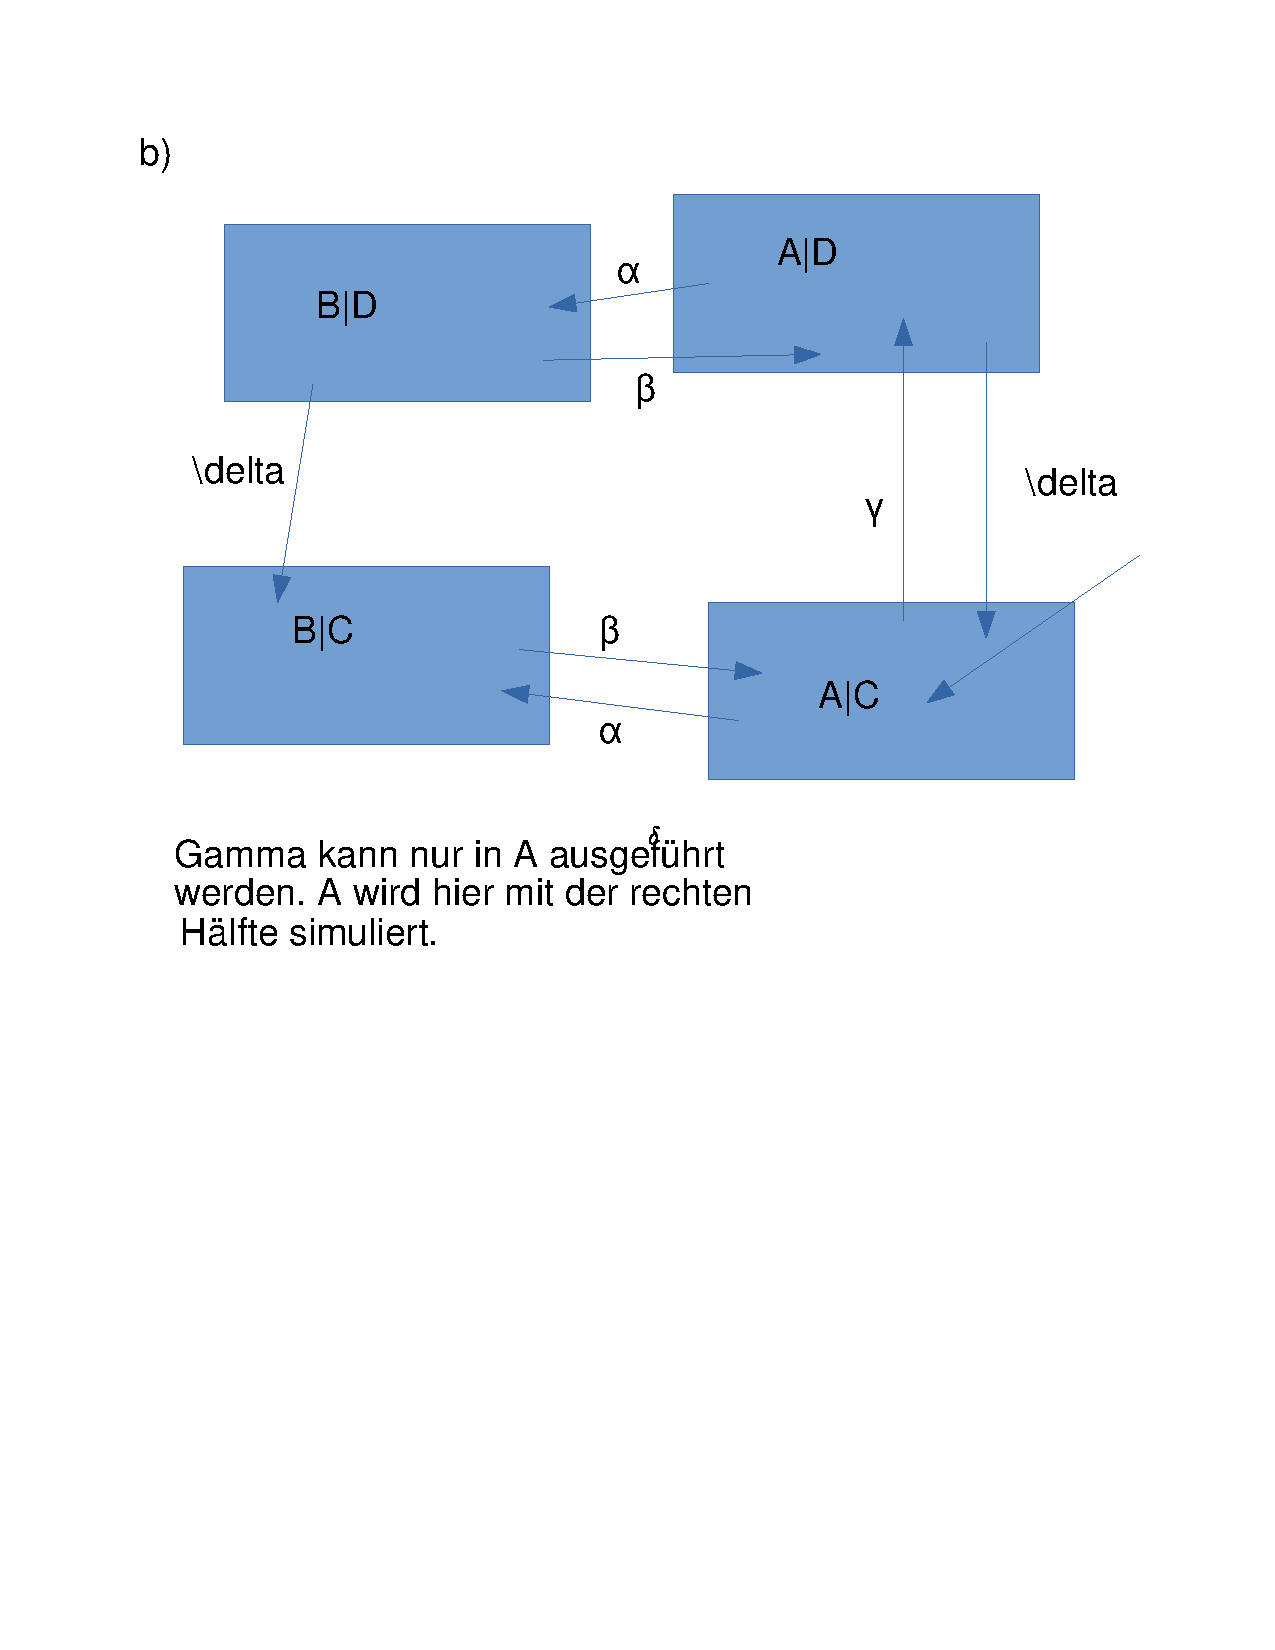
\includepdf[pages=1]{aufgabe1.pdf}
\section*{Aufgabe 2}
Das Erste: \\
Sei $P$ der Anfangszustand.\\
$P := P_{.a.b.c};Q := P_{.a}; R :=Q_{.b}; P:= R_{.c}; R:=P_{.a.b} $ \\

Das Zweite: \\
$Z:= Z_{.x} ; Z :=Z_{.y}$\\


\section*{Aufgabe 3}
Die letzte Seite ist das vollständige Statechart.
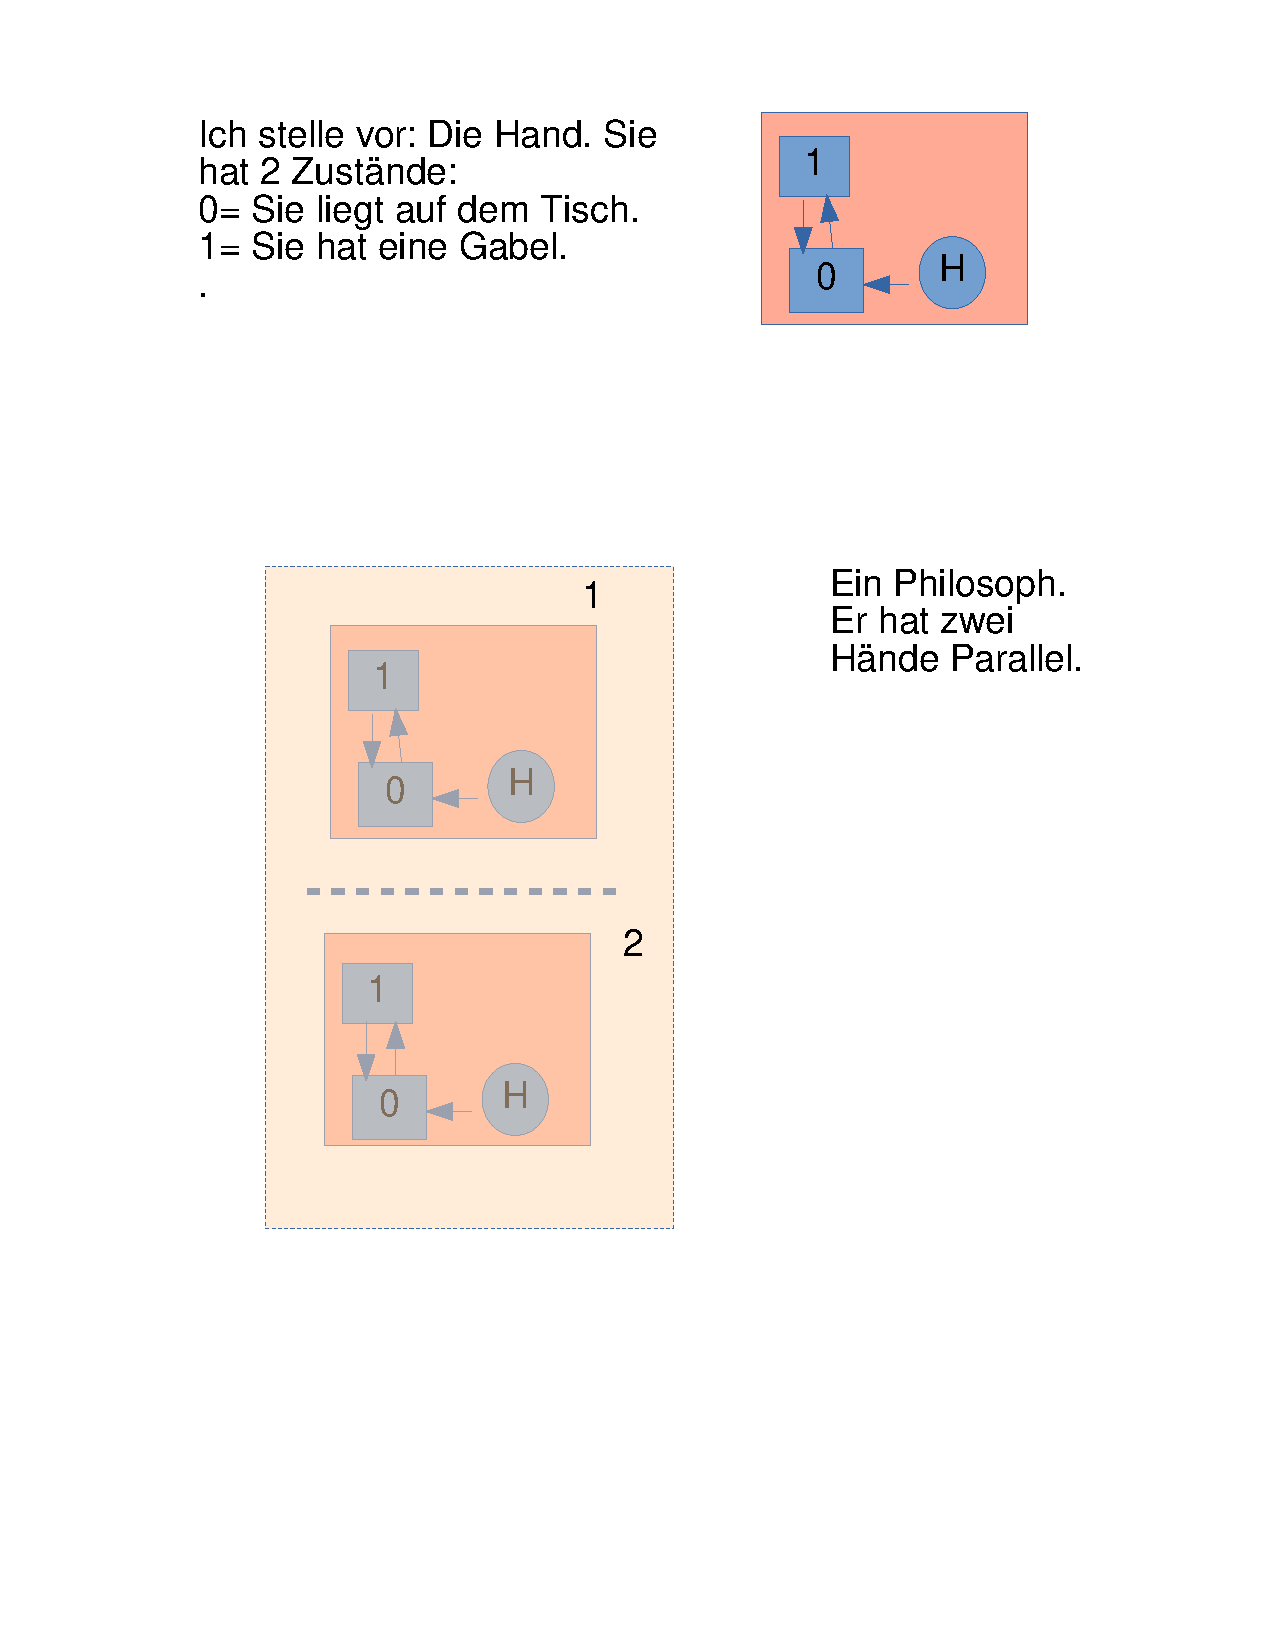
\includepdf[pages=-]{philosophenproblem.pdf}

\end{document}
